\subsection{Opgave 25}

På figuren nedenfor ses grafen for en funktion f.

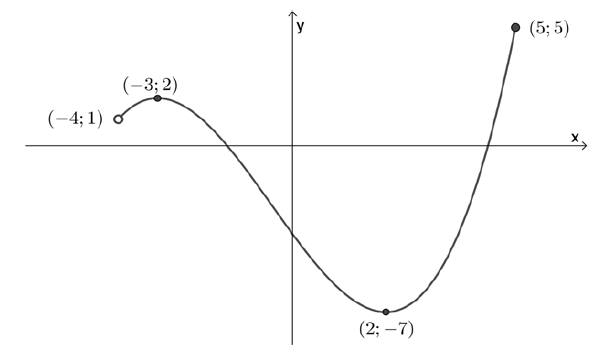
\includegraphics[width=10cm]{Opgave_21-30/Opgave_25/25.png}

Benyt figuren til at bestemme definitionsmængden og værdimængden for funktionen.

\ans

Definitionsmængden for en funktion f (Dm(f)) er alle de tilladte x værdier som funktionen kan have.
Kigger vi på figuren og går langs x-aksen støder vi først på punktet (-4;1). Den laveste x værdi funktionen f kan tage er derfor -4.
Det sidste punkt vi støder på er punktet (5,5). Den højeste x værdi funktionen f kan tage er dermed 5.


Vi opskriver nu definitionsmængden for funktionen f som intervallet mellem dens laveste og højeste x værdi.
Da det første punkt (-4; 1) var åbent hører den laveste x værdi ikke med og den første parentes er derfor åben (vender derfor udad) $\rbrack$.
Da det sidste punkt (5; 5) bar lukket hører den højeste x værdi med og den sidste parentes er derfor lukket (vender indad) $\rbrack$.
Vi får definitionsmængden

\begin{align*}
    Dm(f) = \rbrack-4; 5\rbrack
\end{align*}

Værdimængden for en funktion f (Vm(f)) er alle de tilladte y værdier som funktionen kan have.
Kigger vi på figuren og går langs y aksen fra bunden støder vi først på punktet (2; -7). Den laveste y værdi funktionen f kan tage er dermed -7.
Det sidste punkt vi støder på er punktet (5; 5). Den højeste y værdi funktionen f kan tage er dermed 5.

Vi opskriver nu værdimængden for funktionen f som intervallet mellem dens lavest og højeste y værdi.
Da begge punkterne (2; -7) og (5; 5) er lukkede er begge parenteserne i intervllet derfor lukkede.
Vi får værdimængden

\begin{align*}
    Vm(f) = \lbrack -7; 5 \rbrack
\end{align*}